\documentclass{article}
\usepackage[a4paper, textwidth=14cm]{geometry}
\usepackage{graphicx} % Required for inserting images

\usepackage{hyperref}
\usepackage{cleveref}
\usepackage{listings}

\title{\textbf{Controllable Music Generation}}
\author{Michael Büttner \and Johanna Pries \and David Komnick}
\date{\vspace{-3ex}}
\graphicspath{ {./images/} }


\begin{document}

\maketitle

\section{Introduction}
Music is an important topic for most people in their day-to-day life and we are constantly surrounded by it. But composing music is a very complex art which requires a lot of knowledge. So in addition to human compositions which are made by hand, there is also the approach to generate music via algorithms. For this to be well functioning it is critical to make the music generation controllable. In general, it would be really practical if not the user would have to choose which music they want to listen to, but the music would be automatically chosen based on the mood etc. the user is in at the moment.

Our idea is to generate music depending on the environment or mood a person is currently in. Therefore we need some kind of information about the surroundings of the user. This information should be retrieved by using the data an IMU (Inertial Measurement Unit) system on an Arduino Bluetooth board records. More specifically: the acceleration and orientation of the sensor. This way the generated music can be dynamically adapted to the current environment, without the user having to actively change it.

\section{Methods}
The general idea was to work with successful and promising, already published related work (and file formats) and expand, adapt and improve those approaches for our needs and goals. A substantial part of our work was the modification of FIGARO (FIne-grained music Generation via Attention based, RObust control).

% \subsection{Related work}

\subsection{MIDI}
The MIDI (Musical Instrument Digital Interface) data file format has become a widely adopted standard in the music industry due to its flexibility, efficiency, and controllability. Unlike WAV (Waveform Audio File Format), which represents audio waveforms as raw sampled data, MIDI files store musical information in a symbolic format that encompasses note events, timing, pitch, duration, and other relevant musical parameters. This symbolic representation makes MIDI files highly suitable for controllable music generation with AI.

We decided to use the MIDI data file format instead of the WAV format, because of its inherent advantages in controllable music generation with AI. Another advantage of the MIDI file format is that it is extendable to other formats, such as the the REMI (REvamped MIDI-derived events) \cite{DBLP:journals/corr/abs-2002-00212} and REMI+ \cite{von2022figaro} file format.

\subsection{REMI}
REMI (REvamped MIDI-derived events) was introduced to represent MIDI data following the way humans read them. In addition to the tokens used in the MIDI file format, REMI uses 'Bar' and 'Position' events, indicating the beginning of a bar and the specific position within a bar (quantized to 16 regions), respectively. This structure leads to better rhythmic regularity when modeling music and replaces the need of using a 'Time-Shift' event. In comparison to MIDI, a set of 'Tempo' events was added to REMI to allow for local tempo changes per beat. Additionally, a 'Chord' event was added to make the harmonic structure of music explicit and therefore improve controllability of the chord progression. A chord consists of a root note (C, C\#, D, ...) and a chord quality (major, minor, diminished, ...). Other than in the MIDI format, REMI does not use 'Note-Off' events, but instead uses 'Note Duration' events. Hence, each note is represented with the 'Note Velocity', 'Note-On' and 'Note Duration' event. This gives the advantage, that the duration of a note does not have to be inferred from a time gap and a model does not have to learn that 'Note-On' and 'Note-Off' events must appear in pairs \cite{DBLP:journals/corr/abs-2002-00212}.

\subsection{REMI+}
The original REMI format does not allow for modelling multiple tracks or multiple time signatures. Therefore, REMI+ was introduced as an extension to REMI. REMI+ is suitable for general multi-track, multi-signature symbolic music sequences. This is done by modifications that add time signature and instrument information, determining a unique order of events and use quantization schemes that allow for accurate representation for a diverse set of music \cite{von2022figaro}.

\subsection{FIGARO}
We are using a transformer model for music generation called FIGARO \cite{von2022figaro}. It uses a self-supervised description-to-sequence task to generate symbolic music. There are two kinds of descriptions the model can take as an input. The first one is the expert description (\cref{fig:Figaro}), which includes certain features per bar, such as time signature, note density, mean pitch, mean velocity, mean duration, instruments and chords. It serves as a human interpretable feature description but is only able to capture low-fidelity features.  

The other possible input type is the learned description. It is gained through the use of a Vector Quantized Variational Autoencoder (VQ-VAE) framework. The framework is trained separately to FIGARO and the latent code is used as the learned description. 

The main part of FIGARO is a sequence-to-sequence model which takes either the expert description, the learned description or both as an input and gives music as an output.
The authors of FIGARO proposed and used the REMI+ format. Because of this, we have to convert all inputs from MIDI to REMI+ and all outputs from REMI+ to MIDI. 

\subsection{Training of FIGARO}

\subsection{Modifications to FIGARO}
In order to use FIGARO for our purposes, several parts of the model had to be adapted and extended.

\subsubsection{Experiments with FIGARO}
Since the expert description includes the chords per bar, one idea is to change all the chords to their relative minor or relative major to manipulate the perceived emotion. For example a 'C Major' chord would be rewritten as an 'A Minor' chord and vice versa. This way the musical relations between different chords are conserved in contrast to simply changing the chords to their parallel key (i.e. from major to minor, or the other way around), without adapting the tonic note. But still several other problems are encountered. It is for instance unclear what happens with augmented our diminished chords as those types of chords can be assigned to neither major nor minor scales.

This approach was not further pursued in the project.

\subsubsection{Transformer in FIGARO}
As shown in Figure \ref{fig:Figaro}, FIGARO is build out of two transformers using an encoder-decoder architecture. In the forward-path of FIGARO the hidden state is passed from the encoder to the decoder.

\begin{figure}[h]
\centering
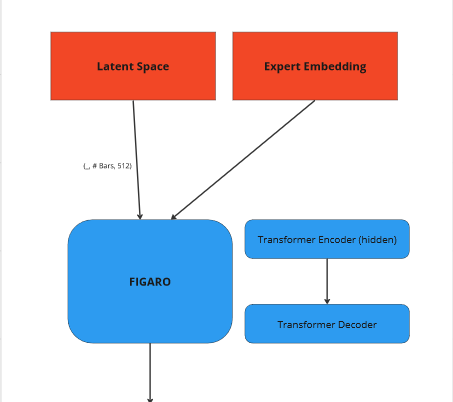
\includegraphics[width=8cm]{Figaro}
\caption{Encoder-decoder architecture of FIGARO (blue) and latent space and expert embedding as input (red).}
\label{fig:Figaro}
\end{figure}

While the encoder is processing a whole bar, the decoder is representing the output token-wise. The look-back of the decoder is (most likely, unless there are many tokens in one bar) more than one bar. The dimensionality of the hidden-state is $(1, \#bars, 256)$.

The entire information about the song is in the hidden state. The idea is to apply a neural network (only containing dense layers as the baseline network) which is tasked to manipulate the hidden state for achieving our conditioned classification goal. We have music of type $c_i$ (in our current case emotions) and we want to change it to music of type $c_j$. How well the transformation worked is determined by our classifier, applied to the REMI+-tokens after applying FIGARO. This is illustrated in Figure \ref{fig:Figaro_trans}.

\begin{figure}[h]
\centering
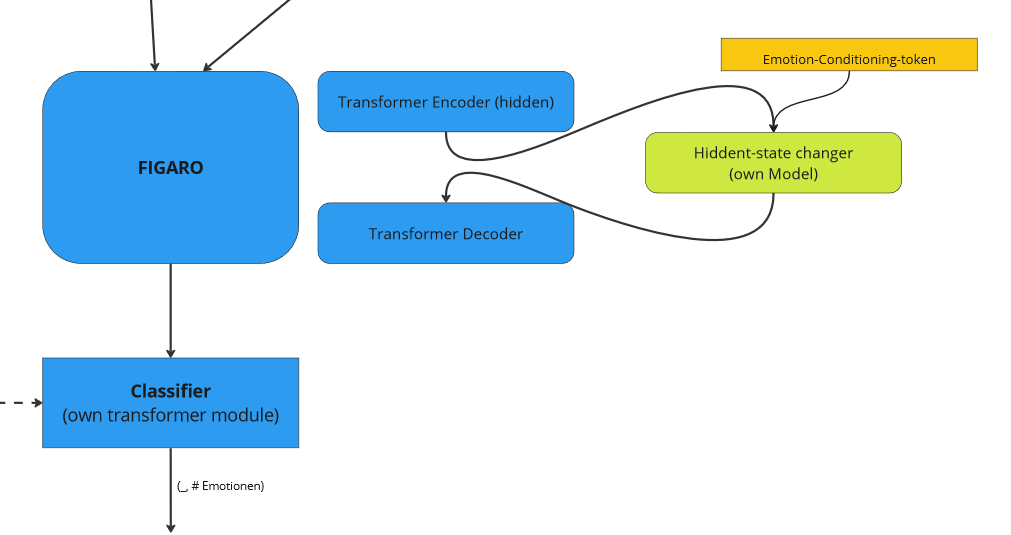
\includegraphics[width=12cm]{Figaro_2}
\caption{FIGARO (blue) with manipulated hidden state (green). After applying FIGARO a classifier is applied to the respective output.}
\label{fig:Figaro_trans}
\end{figure}

Now we want to build a loss function for training our network. We fix the weights of FIGARO and train the green part of Figure \ref{fig:Figaro_trans}. In the original paper (\cite{von2022figaro}) a reconstruction loss is used.
This is not applicable for us since we want to change the output. Therefore it is important to specify our input: The input is a composition of three components:
\begin{enumerate}
    \item The actual song.
    \item The class-label $c$ of the song.
    \item The class-label $y$ we want the output to have.
\end{enumerate}

In general we want to transform the class-label $c$ to $y$ and we can use the categorical cross entropy (assuming an one-hot-vector-encoding). If $c == y$ holds, we want the hidden state to not change at all. In this case we add an identity-loss for the hidden state to our loss function. By this we want to ensure that we do not train $n$ songs, where $n$ is the number of different classes.

We sample from a Conditional Variational Autoencoder (CVAE) which incorporates a conditional variable into both the encoder and the decoder.
% in more detail
The loss function used for training the CVAE is a combination of the Huber loss and the Kullback-Leibler divergence (KLD). The Huber loss is used because it is less sensitive to outliers in data than the squared error loss. As a reduction method for the Huber loss, we used the mean, which leads the sum of the output to be divided by the number of elements in the output. The KLD measures the divergence between one probability distribution and a reference probability distribution (standard normal distribution). Adding the Huber loss to the KLD yields our loss function.

\subsection{Datasets}
In order to train the emotion-classifier, an appropriate dataset is needed. We decided to use the EMOPIA dataset \cite{{EMOPIA}} for this process. EMOPIA is a database including MIDI data which focuses on perceived emotion in pop piano music. The dataset contains 1,087 music clips annotated with emotion labels by hand. The perceived emotions are divided into four quadrants (Q1, Q2, Q3, Q4). These quadrants are defined by the level of valence and the level of arousal (low or high respectively) in the music. We decided to use two of the four quadrants for the training. Quadrant Q1 contains 250 music clips described as high arousal and high valence. The corresponding music is perceived as exciting. Quadrant Q3 includes 253 music clips described as low arousal and low valence. The music in this quadrant is perceived as calm. We chose these two quadrants due to their differences in note density, note length and note velocity.

\subsection{Classifier}
Together with the EMOPIA dataset, several emotion classifiers were introduced and evaluated. The classification task for EMOPIA was defined as classifying a song into one of the four categories (quadrants) described in the section above. For this, the classification results were obtained on symbolic-domain emotion recognition as well as on audio-domain emotion recognition. The symbolic-domain classification includes using two different symbolic note representation methods: MIDI-like and REMI \cite{{EMOPIA}}. For our purposes the symbolic-domain classifier utilizing the REMI input files is suited. 

The model is build as a combination of a bidirectional LSTM and a self-attention module. The temporal information of the songs is extracted by the LSTM. The self-attention module on the other hand computes weight vectors over the hidden states of the LSTM  with multi-head attention. Eventually, the resulting weighted hidden states are used for the classification \cite{{EMOPIA}}.

For our work this classifier can be repurposed but first has to be adapted to REMI+ in order to do so.

\section{Arduino board with integrated IMU}
To generate music based on an environment, we have to collect environmental data and transform them into a format that can be used to guide the generation process.

\subsection{Collection of raw data}
We use an Arduino board to collect raw environmental data. Arduino is an open-source electronics platform based on easy-to-use hardware and software \cite{arduino}. It is compatible with Linux, Mac and Windows systems. Arduino boards are able to read inputs from various sensors and turn them into outputs. It is possible to upload scripts to the microcontroller to control the behavior of an Arduino board.

For this project the Arduino Nano 33 BLE Sense Rev2 is used \cite{arduinoBLE}. It is equipped with an IMU (Inertial Measurement Unit) featuring an accelerometer, a gyroscope and a magnetometer, as well as with a microphone and sensors for measuring light, barometric pressure and temperature. The board can be connected to a computer via Bluetooth Low Energy so that the produced outputs can be read and recorded for further use.

The Arduino board was configured by us to enable transmissions between the board and a computer. We use a sketch published by Arduino with modifications for the Rev2 hardware \cite{arduinoSketch}. After uploading the sketch to the Arduino board using the Arduino Software IDE, the board is sending out sensor data on different channels.

\begin{lstlisting}[language=C, frame=single, breaklines=true]
BLEService                     service                       (BLE_SENSE_UUID("0000"));
BLEUnsignedIntCharacteristic   versionCharacteristic         (BLE_SENSE_UUID("1001"), BLERead);
BLEUnsignedShortCharacteristic ambientLightCharacteristic    (BLE_SENSE_UUID("2001"), BLENotify); // 16-bit
BLECharacteristic              colorCharacteristic           (BLE_SENSE_UUID("2002"), BLENotify, 3 * sizeof(unsigned short)); // Array of 16-bit, RGB
BLEUnsignedCharCharacteristic  proximityCharacteristic       (BLE_SENSE_UUID("2003"), BLENotify); // Byte, 0 - 255 => close to far
BLEByteCharacteristic          gestureCharacteristic         (BLE_SENSE_UUID("2004"), BLENotify); // NONE = -1, UP = 0, DOWN = 1, LEFT = 2, RIGHT = 3
BLECharacteristic              accelerationCharacteristic    (BLE_SENSE_UUID("3001"), BLENotify, 3 * sizeof(float)); // Array of 3 floats, G
BLECharacteristic              gyroscopeCharacteristic       (BLE_SENSE_UUID("3002"), BLENotify, 3 * sizeof(float)); // Array of 3 floats, dps
BLECharacteristic              magneticFieldCharacteristic   (BLE_SENSE_UUID("3003"), BLENotify, 3 * sizeof(float)); // Array of 3 floats, uT

BLEFloatCharacteristic         pressureCharacteristic        (BLE_SENSE_UUID("4001"), BLERead); // Float, kPa
BLEFloatCharacteristic         temperatureCharacteristic     (BLE_SENSE_UUID("4002"), BLERead); // Float, Celcius
BLEFloatCharacteristic         humidityCharacteristic        (BLE_SENSE_UUID("4003"), BLERead); // Float, Percentage
BLECharacteristic              microphoneLevelCharacteristic (BLE_SENSE_UUID("5001"), BLENotify, 32); // Int, RMS of audio input
BLECharacteristic              rgbLedCharacteristic          (BLE_SENSE_UUID("6001"), BLERead | BLEWrite, 3 * sizeof(byte)); // Array of 3 bytes, RGB
\end{lstlisting}

The output of the Arduino board is collected using a Python script. With the async and the bleak library, we can search for Bluetooth devices and read the data transmitted by them using \texttt{BleakScanner.discover()}. After a successful connection, we can search for a specific channel to read out data from a certain sensor. A showcase of this process can be found at our GitHub repository \cite{getGyro}. The received data are written into files at last.

\begin{lstlisting}[language=Python, frame=single, breaklines=true]
async def main():
    devices = await BleakScanner.discover()
    adress = ""
    found = False
    for d in devices:
        if d.name == "IMU1":
            adress = d.address
            found = True
        print(d)
    if found:
        async with BleakClient(adress) as client:
            print("Gyroscope found!")
            await client.start_notify(uuid_gyro_service, notification_handler)
            if(len(sys.argv) > 1 and sys.argv[1] == "endless"):
              while(1):
                  await asyncio.sleep(10.0)
            else:
                await asyncio.sleep(10.0)
            await client.stop_notify(uuid_gyro_service)
    else:
        print("Gyroscope not found!")    
\end{lstlisting}

\subsection{Processing of the data}
A first concept is to record a specific sensor value for a certain period of time, e.g. the gyroscope angles for the X, Y and Z axis. The mean and standard deviation values can be used to determine whether the Arduino board is in movement, indicating a higher activity in the environment. Further sensor data can be collected to support or modify the results. For example a high velocity detected by the accelerometer indicates high energy, while low volume detected by the microphone suggests a rather quiet and relaxed environment. These values are included in the computation, which results in a certain emotion for the to be generated music.


\section{Discussion}

\subsection{Future Work}
Our work does not have to be limited on emotion related tasks. It could be adapted to several other domains. Instead of a dataset classified based on emotion, for example a dataset divided into different genres of music could be used.

Generally, to improve the results, different kinds of music clips could be chosen. It could be potentially beneficial to use simple and not too complex music clips to improve the quality of the generated music.

\subsection{Conclusion}

\bibliographystyle{ieeetr}

\bibliography{citation} 

\end{document}

